\chapter{Analysis technique}
\label{chap:Reconstruction}

\chapterquote{In preparing for battle I have always found that plans are useless, but planning is indispensable.}%
{Dwight D. Eisenhower}%:

Automated analysis is the only way to deal with the vast amount of data generated in the high energy physics. In the last chapter we described the automated reconstruction tools in details. This chapter is dedicated to the common automated analysis tools and techniques, which will be used in the analysis described in subsequent chapters.

For the linear collider, thanks to the high granular calorimeter, the starting point for analysis would be individual Particle Flow Objects, as well as individual tracks. Each of the PFOs encodes four-momentum and position information. For tracks, they would have momentum and position information.

However, sometimes it is interesting to group PFOs and tracks into jets, where a jet is the result of hadronisation process from high energy particles like quarks or gulons.
\begin{comment}
\section{Jet algorithm}

A jet is typically a visually obvious structure in a event display. The momentum and the direction of a jet tend to resemble the originated particle. Despite the relative easiness of identifying jets visually, it presents a challenge for a pattern recognition program to identify jets effectively and efficiently.

Early work on jet finding started in 1977 \cite{PhysRevLett.39.1436}, where later development can be found in reviews \cite{Moretti:1998qx,Salam:2009jx,Ali:2010tw}.

There are two large families of jet finding algorithm, cone based algorithm, and sequential combination algorithm. Cone based algorithm is briefly discussed in \Section{sec:pandoraConeClustering}.

Sequential combination algorithm typically calculate a pair-wise distance metric. Pairs with the smallest metric will be combined. The metric will be calculated and updated, and a pair with smallest metric will be combined. This procedure will be repeated until some stopping criterion are satisfied.

The chosen jet algorithm implementation is FastJet C++ software package \cite{Cacciari:2011ma,Cacciari:2005hq}, providing a wide range of jet finding algorithms. The implementation in Marlin software package is called MarlinFastJet. The symbols in the subsequent discussion about specific jet algorithms will follow \cite{Cacciari:2011ma}

\subsection{\kt algorithm}

One of the common sequential combination algorithms for \pp collider experiment, is longitudinally-invariant \kt algorithm \cite{Catani:1993hr,Ellis:1993tq}. In the inclusive variant, The symmetrical pair-wise distance metric between particle $i$ and $j$, and the beam distance, are defined as
\begin{equation}
&d_{ij} = d_{ji} = \min\!\parenths{\pT_{i}^{2},\!\pT_{j}^{2}}\frac{\DeltaOf{R_{ij}^{2}}}{R^{2}}, \\
&d_{iB} = \pT_{i}^2,
\end{equation}
where $\pT_{i}$ is the transverse momentum of particle $i$ with respect to the beam ($z$) direction, and $\DeltaOf{R_{ij}^{2}}$ is the measurement of angular separation of particle $i$ and $j$. Formally $\DeltaOf{R_{ij}^{2}} = \parenths{y_i - y_j}^2 + \parenths{\phi_i - \phi_j}^2$, where $y_i = \frac{1}{2}\ln\!\frac{E_i + {p_z}_i}{E_i - {p_z}_i}$ and $\phi_i$ are particle $i$'s rapidity and azimuthal angle. R is a free parameter controlling the jet radius.

If $d_{ij} < d_{iB}$, particle $i$ and $j$ are merged, with the \fourMomentum of particle $i$ updated as the sum. Otherwise, particle $i$ is set to be a final jet, and delete from the particle list. The above procedure is repeated until no particle left.

The exclusive variant is similar. First difference is that when  $d_{iB} < d_{ij}$, the particle $i$ is discarded and part of the beam jet. The second difference is that when both $d_{ij}$ and $d_{iB}$ are above some threshold, $d_{cut}$, the clustering will stop. In practise, exclusive mode allows a specified number of jets to be found, which will automatically choose the $d_{cut}$. The inclusive mode would fine as many jets as the algorithm allows.
\end{comment}
\subsection{Durham algorithm}

Durham algorithm \cite{Catani:1991hj}, also known as \ee \kt algorithm, is commonly used \ee collider experiment. It has a single distance metric:
\begin{equation}
d_{ij} = 2\min\!\parenths{E_i^2,\!E_j^2}\!\parenths{1 - \cosOf{\theta_{ij}}},
\end{equation}
where $E_i$ is the energy of particle $i$. $\theta_{ij}$ is the polar angle difference between particle $i$ and $j$. Durham algorithm can only be run at exclusive mode, which means that the clustering will stop when $d_{ij}$ is above some threshold, $d_{cut}$.

Comparing to \kt algorithm, it uses energy instead of \pT in the distance metric, and it did not have a beam jet. This is because that for the \ee collider in the past, the beam induced background was not severe and collisions energy is known, \sqrtS.
\begin{comment}
\subsection{Jet algorithm for \CLIC}

Although \CLIC is a \ee collider, the significant beam-induced background adds a large amount of energy from \ggHad process. Therefore, traditional \ee jet algorithms, like Durham algorithm, is not suitable for \CLIC environment. Studies has shown that jet algorithms for \pp collider have better performance \cite{Linssen:2012hp,LCD-Note-2010-006}.

A more recent attempt at marrying merits from both Durham and \kt algorithms has resulted in Valencia jet algorithm \cite{Boronat:2014hva}. It had shown promising improvement comparing to \kt algorithm.

\begin{comment}
Why extra C++ implementation
speed reduce O(n^3) to NlgN
y, phi space, 2D KNN problem
\end{comment}

\subsection{\y{} parameter}
\y{} parameter is a commonly used quantity to describe the transition of exclusive jet algorithm going from $N$ clustered jets to $N\!+\!1$ clustered jets. For example, $\y{23}$ would be the $d_{cut}$ value for a exclusive jet algorithm, above which the jet algorithm returns 2 jets, below which the jet algorithm returns 3 jets.

Numerically \y{} parameter is often much smaller than one. A typically way to convert the small number to a human acceptable range is to take the minus logarithm of the number.
\begin{comment}
\section{Flavour tagging}
\label{sec:theoryFalvourTagging}

The latest software package for jet flavour tagging is \lcfiplus \cite{Suehara:2015ura}. It is based on the LCFIVertex package, which was used in the simulation studies for \ILCloi \cite{Abe:2010aa,Aihara:2009ad} and \CLICcdr \cite{Linssen:2012hp}. Current software is built in mind of a future \ee collider. Although the software is modular, it will be described in order that it will be used in a physics analysis,

The vertex finding algorithms perform vertex fitting and identify primary and secondary vertex. There is a ``V0'' particle rejection, which is when neutral particles decay or convert into a pair of charged tracks. The topology is similar to the decay of \Pbottom or \Pcharm hadrons. Hence it is important to remove the V0 particles to improve the heavy quark falvour tagging.

Jet clustering ensures that the secondary vertices and the muons identified from semileptonic decay are combined. Therefore, it is consistent with the hadronic decay. Jet algorithms used are Durham and Durham modified algorithms.

Vertices are refined to improve the \Pbottom jet identification from c jet. Two vertices is strongly correlated to a \Pbottom jet. Hence the vertices refining will reconstruct as many secondary vertices correctly as possible.

The final flavour tagging of the jet is done using multivariate analysis, which will be discussed in \Section{sec:theoryMVA}. Using TMVA software package \cite{Hocker:2007ht}, Boosted Decision Tree classier is used. A series of flavour sensitive variables are calculated, and the classification is divided four sub-set: jet with zero, one, or two properly reconstructed vertices, or a single-track pseudovertex. For each sub-set, a jet can either be a \Pbottom jet, a \Pcharm jet, or a light flavour quark jet (\Pup, \Pdown or \Pstrange). The multiclass classifier's response is normalised across different sub-set, and they will be referred in the subsequent physics analysis as the tag value.
\end{comment}
\section{Multivariate analysis}
\label{sec:theoryMVA}

Multivariate analysis (MVA) has become increasingly common in high energy physics. MVA can be viewed as an advanced tool for regression or classification. Comparing to the traditional cut based method, modern machine learning technique offers much improvement in data analysis.

Software package for MVA used throughout this document is TMVA \cite{Hocker:2007ht}.

A typical machine learning MVA classification involves two classes, also known as signal and background. A machine learning model, called classifier in TMVA, needs to be trained with training data. The model requires a set of discriminative variables, which should separate signal from background. The trained model will be applied onto the testing data, for signal extraction. Response of the model could be signal/background, or be  a number in a continuous spectrum, where the user decides the value to separate signal from background.

Strictly, there should be three statistically independent samples for the MVA. One sample is for the training. Another sample for the validation, including optimisation and checking for overfitting. The last sample is for testing. However, due to technical reason, sometimes the same sample is used for the validation and the testing.

This classification scheme can be easily extended to multiple classes, implemented in TMVA with multiclass class.

\subsection{Optimisation and overfitting}

The optimisation of the model is to select the optimal free parameters of the model. One could build a complex model which fits the training samples very well, but it would not be optimal for another testing sample. A simple model is less prone to statistical fluctuation of samples, however, it might be too simple to achieve the optimal modeling. The former case is known as overfitting, or overtraining. The latter case is called underfitting, or undertraining.

The compromise is clear. The optimal model is one between overfitting and underfitting. In practice, this involves building the model with increasing complexity, and finding the point where overfitting occurs.

\begin{figure}[!tbp]
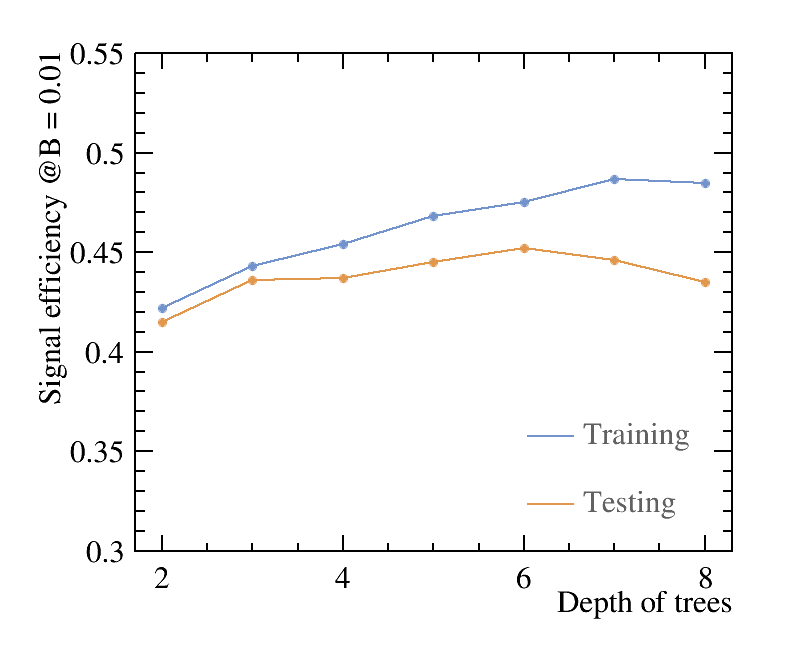
\includegraphics[width=\largefigwidth]{doubleHiggs/DepthOfTrees}
\caption[MVA overtraining]%
   {MVA overtraining}
   \label{fig:analysisMVAovertraining}
\end{figure}

\Figure{fig:analysisMVAovertraining} shows a typical overfitting plot. Overfitting is defined when the efficiency of signal selection in the training samples increases, but the efficiency in the testing sample decrease. Here the example is chosen from double Higgs analysis, using Boosted Decision Tree model, for \rootS{3} samples. The efficiency of signal selection is defined as the signal efficiency when background efficiency is 1\%, report by the TMVA training process. In the plot, the depth of the tree, or the number of layers in the tree, reflects the complexity of the model. From tree depth 2 to 5, the efficiency for both testing and training samples increases. From tree depth 6 onwards, the overfitting occurs. In this particular example, one should choose a tree depth fewer than 7 to avoid overfitting.

There are methods to assign the error on the selection efficiency. Thus one can make a better choice of parameters to avoid overfitting. These methods were not implemented due to the technical capacity provided by the TMVA.

\subsection{Choice of models}

The model, known as the classifier in TMVA, can be as simple as cut based, likelihood or linear regression. It can be complicated as non linear tree, non linear neutral network or support vector machine. Regardless of model complexity, the choice of most optimal classifier is often data driven. Also, given the free parameters in each model, the comparison between different models without individual tuning is not rigorous. Nevertheless, as researchers in the machine learning suggested, the boosted decision tree is probably the best out-of-the-box machine learning method. Neutral network could potentially be better than the boosted decision, but it requires more tuning, and it is less intuitive to interpret the model. For these reasons, boost decision tree (BDT) is often the choice of machine learning model in the high energy physics. And it is used in various physics analysis in this document.

Before describing BDT in detail, we will first visit the traditional rectangular cut model, and the Projective Likelihood method, which is used in the photon ID in the \pandora.



\subsection{Rectangular Cut}

Probably the most intuitive model, the rectangular cut method optimise cuts to maximise some specific metric. The metric could be the signal efficiency for a particular background efficiency. Alternatively, the metric can be the significance, $\frac{S}{\rootOf{S\!+\!B}}$, where $S$ and $B$ are signal and background numbers, respectively.

Discriminative variables gives better separation power when they are gaussian-like and statistically independent. Therefore it is common to decoorelate  the variables and gaussian transform them before using the rectangular cut MVA.

Because its simplicity, the cut method is often performed manual, much more often in the time pre-date the wide spread of machine learning methods. It is still commonly used for the pre-selection step before the MVA, and other simple usages. Unless specified, the optimal cuts proposed in this document for various physics analysis are found using the rectangular cut method manually.

\begin{comment}
\subsection{Projective Likelihood}

Projective likelihood model (PDE) is used in \pandora for the photon ID due to its simplicity and low requirement on computing resources.

PDE implemented in the TMVA calculates the probability density for each discriminative variable, for signal and background. The overall signal and background likelihood are defined as products of the individual probability density. The likelihood ratio, $R$, is then defined as the signal likelihood over signal plus background likelihood.

TMVA implementation also fits an underlying function to the probability density. The \pandora implementation simply uses binned likelihood ratio, $R$, as the output, due to the simplicity. The sub-categories for the \pandora implementation are determined by the cluster energy.

Similarly to the rectangular cut method, PDE works better with decorrelated, gaussian like variables. The \pandora implementation did not decorrelate nor transform the variables, to keep implementation fast.
\end{comment}

\subsection{Boosted decision tree}
\label{sec:analysisBDT}
Boost decision tree (BDT) is a non linear tree based model. Its rather complex nature requires a careful explanation of many concepts within the BDT.

Decision tree is a binary tree, where each node, the splitting point, uses a single discriminative variable to decide whether a event is signal-like (``goes down by a layer to the left''), or background-like (``goes down by a layer to the right''). At each node, samples are divided into signal-like and background-like sub-samples. The tree growing starts at the root node, and stops at certain criterion, which could be the minimum number of events in a node, the number of layers of the tree, or a minimum/maximum signal purity.

The training of the decision tree is to determine the optimal cut at the node. The the probability of the cut produces the signal is $p$. Three commonly used metrics for two-class classification are
\begin{enumerate}
\item Misclassification error:  $1 - \max\parenths{p\!,\!1\!-\!p}$,
\item Gini index: $2p\parenths{1\!-\!p}$,
\item Cross-Entropy or deviance: $-p\log{p}-\parenths{1\!-\!p}\log\parenths{1\!-\!p}$.
\end{enumerate}

The using of a trained decision tree is to transverse along the tree. The event is classified as signal or background depending on whether it falls in the signal-like or background-like end node.

Decision tree has a low bias, but high variance. This means it is very easy to construct a tree that fits the training data very well, but the tree would not be optimal for the testing sample. To overcome the instability of the decision tree, many methods have been developed. The most successful one is boosting.

Boosting: it is a technique where the misclassified events receives a higher weight than the correctly classified events. Therefore, when the training is iterated, the misclassified events would receive higher and higher wights and more likely to classify correctly. The boosting is done at every iteration, which can be few hundred or few thousand time. This will create a ``forest'' of many trees. The final output could be a majority vote, by transversing the event to the end node for each tree in the forest.

Bagging: also known as boot-strap, it is a method that select a simple random sub-set of the training sample, and apply the model. In this case, every boosting iteration takes a bagged sample, rather than the whole sample.

TMVA implementation of the BDT for the output is using a likelihood estimator, depending on how often a event is classified as signal in the forest. The likelihood number is later used to select signal from background.

\subsection{Optimisation of Boosted decision tree}

Many parameters can be tuned. Hence we dedicate a small section to describe the tuning parameters.

The most important parameter is the depth of a tree, which determines how many end nodes a tree has, or the degrees of freedom of a tree. The related parameter is the number of trees. Experience shows that using many small trees yields the best result.

The minimum number of events in a node, which is a stopping criteria for tree growing, affects the size of the tree. But it is less influential than the depth of the tree.

The learning rate, which controls how fast the weight changes for events in each boosting iteration. Experience shows small learning rate with many trees work better than large learning rate with few trees.

The usual choice of the metric for the optimal cuts is either Gini index or cross-entropy. (See \Section{sec:analysisBDT}) We chose Gini index for out BDT usages, as it makes little difference to performances, comparing to the cross-entropy metric.

Number of bins per variables for the cut is necessary to make tree growing efficient. Discrete binned variables are faster to computer than continuous variables. The parameter does not impact the performance much. However, variables should be pre-processed before going into the model. For example, the variable should be limited to a sensible range to avoid the extremes. The variable should also be transformed to obtain a more uniform distribution, if the original distribution is highly skewed.

The boosting has two variant, adaptive boost and gradient boost. For all the BDT used in this document, adaptive boost is used.

For the end node, it is determined as either signal-like or background-like, based on the majority for the training event in the end node. Numerically, it corresponds to 1/0. However, the end node could also use signal purity as the output, resulting in a continues spectrum of [0,1].


\subsection{Multiple classes}
% ATTN used in tau chapter
\begin{comment}
The above discussion is done assuming two classes - signal and background. The argument can be easily extended to multiple classes. There are two ways for the training. "One v.s. one" is each class is trained against each other class. And the overall likelihood is normalised. The second way to train is called "one v.s. all", which is when each class is trained against all other classes.

Using a three-class example, A, B and C, "one v.s. one" scheme trains A against B, B against C, and C against A. Then the likelihood is normalised. "One v.s. all" would train A against B plus C, B against A plus C, and C against A plus B.

TMVA multiclass implementation uses "one v.s. all" scheme. Multiclass is used in falvour tagging of jets, \Section{sec:theoryFalvourTagging}, and in the tau lepton final state separation study, \Section{}.
\end{comment}
\section{Event shape varaibles}

% ATTN used in tau chapter
\begin{comment}
Event shape variables are some useful global variables to describe the shape of the event, for example whether it is back-to-back, or homogenous in the solid angle.

The classical event shape thrust\cite{PhysRevLett.39.1587}, is defined as
\begin{equation}
T = \max_{\hat{t}}\!\frac{\sum_{i}\absOf{\hat{t}\!\cdot\!\vec{p_{i}}}}{\sum_{i}\absOf{\vec{p_{i}}}}
\end{equation}
where $\vec{p_{i}}$ is the momentum vector of the particle $i$. Summation is over all particles in the event. Thrust axis, $\hat{t}$, is a unit vector. (Principle) Thrust value, $T$, is 1 for a perfect pencillike back-to-back two-jet event, and 0.5 for a perfect spherical event. The thrust value is useful in picking out back-to-back two-jet event. Thrust axis is useful to separate each jet in a back-to-back two-jet event.
\end{comment}
\begin{comment} in double higgs
Sphericity tensor \cite{PhysRevLett.35.1609}, is defined as
\begin{equation}
\bm{S^{\alpha\beta}} = \frac{\sum_{i}p^{\alpha}_{i}p^{\beta}_{i}}{\sum_{i}\absOf{\vec{p_{i}}}^2},
\end{equation}
where $\vec{p_{i}}$ is the momentum vector of the particle $i$. Summation is over all particles in the event. $\alpha$ and $\beta$ refer to the x, y, z coordinate axis. Eigenvalues of tensor $\bm{S}$ can be found, or in this case diagonalisation of the matrix $\bm{S}$, denoted with $\lambda_{1}$, $\lambda_{2}$, $\lambda_{3}$. The normalisation condition requires $\lambda_{1}\!\geqslant\! \lambda_{2} \! \geqslant \! \lambda_{3}$ and $ \lambda_{1} \! + \! \lambda_{2} \! + \! \lambda_{3} \! = \! 1 $. Sphericity, $S$, is defined in terms of $\lambda$,
\begin{equation}
S = \frac{3}{2}\parenths{\lambda_{1} \! + \! \lambda_{2}}.
\end{equation}
$S$, is 0 for a perfect pencillike back-to-back two-jet event, and 1 for a perfect spherically symmetric event.
\end{comment}
Aplanarity is another event shape varaible that distinguishes spherical symmetrical events from planar and linear events. The definition is
\begin{equation}
S = \frac{3}{2}\parenths{\lambda_{1}},
\end{equation}
where $\lambda_{1}$ is the largest eigenvalue in the diagonalised sphericity tensor.

\section{Miscellaneous}

An event in a collider experiment refers to one collision and the subsequent energy deposition in the detector. An event corresponds to a certain type of physics process.

Often we are dealing with extracting a type of events, from a large number of other events. The signal, or signal events refer to events of interests. Other events are referred to as the background, or background events.

Typical metrics of signal selection is efficiency and purity. This toy example illustrates definitions of efficiency and purity.

\begin{table}[!tbp]
\begin{tabular}{lrr}
\hline
\hline
Event Number  &  True Signal & True Background  \\
\hline
Selected Signal & $N_S$ & $N_1$ \\
Selected Background & $N_2$ & $N_B$ \\
\hline
\hline

\end{tabular}
\caption[A toy example to demonstrate definitions of efficiency and purity.]%
    {A toy example to demonstrate definitions of efficiency and purity.}
\label{tab:analysisToyExample}
\end{table}
Signal selection efficiency is defined as $\frac{N_S}{N_S \! + \! N_2}$. Signal selection purity is defined as $\frac{N_S}{N_S \! + \! N_1}$.
Significance is a quantity that is similar to purity, $\frac{N_S}{\rootOf{N_S \! + \! N_1}}$

When we are describing particles, light lepton, \llight, refer to electrons, \Pem, and muons, \Pmuon. Light quarks, \qlight, refer to up quark, \Pup, down quark, \Pdown, and strange quark, \Pstrange.

Computational intensive jobs are processed either on the Cambridge High Energy Physics grid, or the \CLIC computing grid.
%Thanks computing resources. i.e. ILC VO, CLIC grid, etc. 